% -----------------------------------------------------------------
% Desenvolvido por Filipe Fernandes para o LIPES (Laboratório de Inovação, Pesquisa e Engenharia de Software)
% filipe.fernandes@ifsudestemg.edu.br
% ----------------------------------------------------------------
% Adaptado de Template Latex - Apresentação - UFMG
% https://www.overleaf.com/latex/templates/template-latex-apresentacao-ufmg/ygvvbrrsqgkv
% -----------------------------------------------------------------
% Licença Creative Commons CC BY 4.0
% -----------------------------------------------------------------
% PARA CORRER pdflatex -shell-escape main.tex
\documentclass[aspectratio=169,english]{beamer}

% a opção hideSubsectionTitle esconde o título das subseções
\usepackage{templateLIPES}      % o arquivo templateLIPES.sty possui todo o estilo de formatação
\usepackage[spanish]{babel}     % mude o idioma, caso necessite
\usepackage[alf, abnt-emphasize=bf, abnt-etal-text=it]{abntex2cite}

\setbeamertemplate{bibliography item}{}
\renewcommand{\theenumiv}{}

\begin{document}

\titulo{Incorporación de técnicas de muestreo mediante histogramas multidimensionales al código de
simulación de fuentes de Monte Carlo KDSource}
% \subtitulo{Subtítulo}       % caso não haja, comente

\autor{Lucas Ezequiel Ovando}
\orientador{Dr. Ariel Marquez}        % caso não haja, comente
\coorientador{Ing. Zoe Prieto}      % caso não haja, comente

\juradoA{Dr. Edmundo Lopasso}
\juradoB{Mg. Norberto Schmidt}

\curso{Ingeniería Nuclear}

\local{San Carlos de Bariloche, Río Negro, Argentina}
\dia{5}
\mes{marzo}
\ano{2025}

% NÃO REMOVA!
\begin{frame}[plain]
    
    \begin{tikzpicture}[overlay,remember picture]
        \node[left=-0.15cm] at (current page.0){
            
\includegraphics[scale=0.145]{imagens/capaLIPES}
        };
    \end{tikzpicture}

    \titlepage
    
\end{frame}

\section[Resumen]{}

\begin{frame}[allowframebreaks]
    \frametitle{Resumen}
    \tableofcontents
\end{frame}

% CONTEÚDO -----------------------------------------------------------------

\section{Introducción}
% \begin{frame}{Motivación}
%     \begin{figure}
%         \centering
%         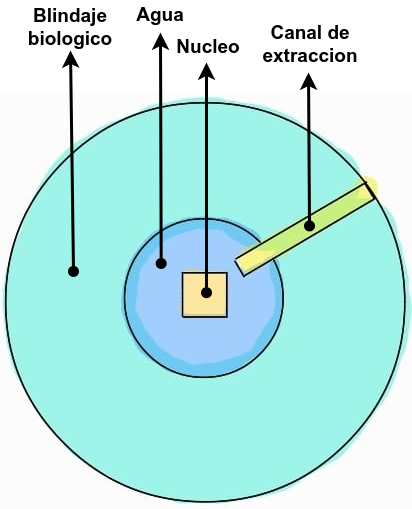
\includegraphics[width=0.35\linewidth]{imagens/nucleo1.png}
%         % \caption{1º seminário do LIPES em 27/01/2025}
%         % \label{fig:esquema1}
%     \end{figure}
% \end{frame}

\begin{frame}{Motivación - Simulación en 1 etapa}
    \begin{figure}
        \centering
        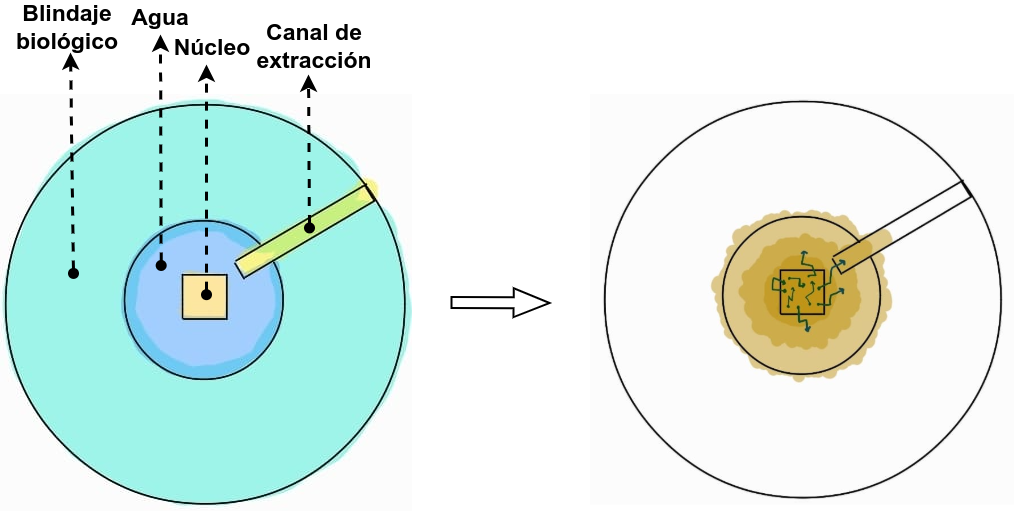
\includegraphics[width=0.85\linewidth]{imagens/nucleo2.png}
        % \caption{1º seminário do LIPES em 27/01/2025}
        % \label{fig:esquema1}
    \end{figure}
\end{frame}

\begin{frame}{Motivación - Simulación en 1 etapa}
    \begin{figure}
        \centering
        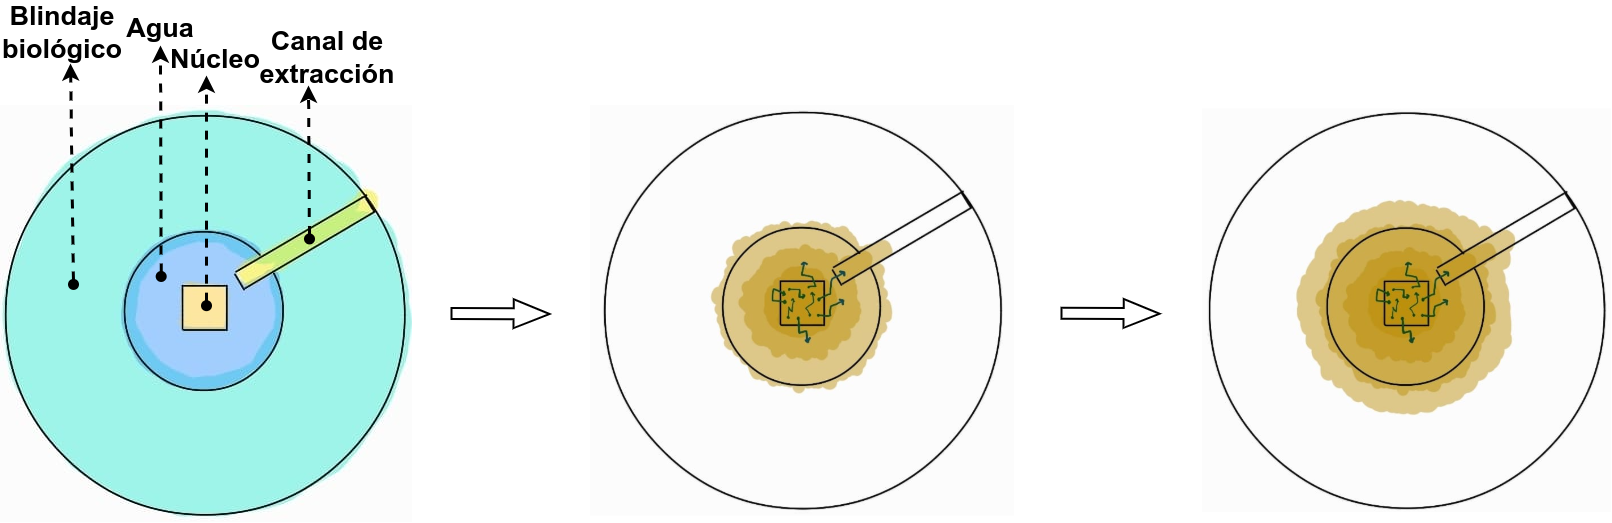
\includegraphics[width=1\linewidth]{imagens/nucleo3.png}
        % \caption{1º seminário do LIPES em 27/01/2025}
        % \label{fig:esquema1}
    \end{figure}
\end{frame}

% \begin{frame}{Motivación - Simulación multi etapas}
%     \begin{figure}
%         \centering
%         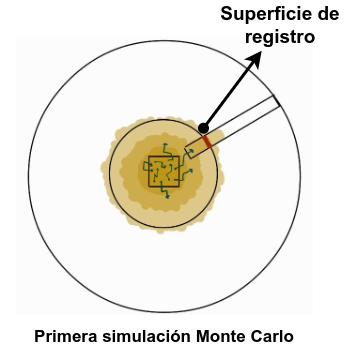
\includegraphics[width=0.45\linewidth]{imagens/nucleo6.png}
%         % \caption{1º seminário do LIPES em 27/01/2025}
%         % \label{fig:esquema1}
%     \end{figure}
% \end{frame}

\begin{frame}{Motivación - Simulación en múltiples etapas}
    % \begin{minipage}{\textwidth}
    %     \hspace{1cm}  % Ajusta la posición horizontal
    %     \vspace{cm}  % Ajusta la posición vertical
    %     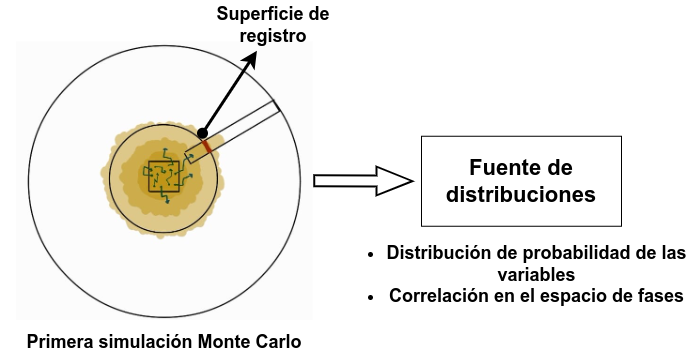
\includegraphics[width=0.85\linewidth]{imagens/nucleo5.png}
    %     % \caption{1º seminário do LIPES em 27/01/2025}
    %     % \label{fig:esquema1}
    % \end{minipage}

    \begin{figure}
        \centering
        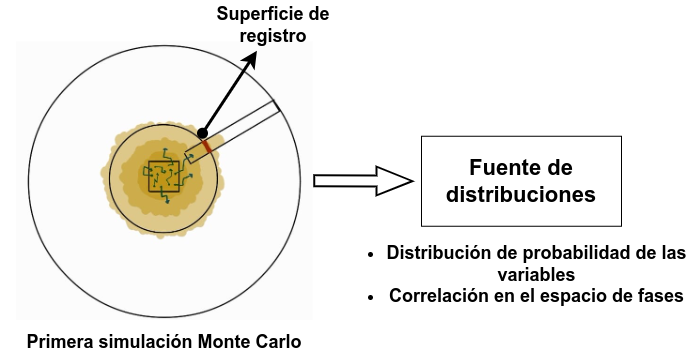
\includegraphics[width=0.83\linewidth]{imagens/nucleo5.png}
        % \caption{1º seminário do LIPES em 27/01/2025}
        % \label{fig:esquema1}
    \end{figure}
\end{frame}

\begin{frame}{Motivación - Simulación en múltiples etapas}
    \begin{figure}
        \centering
        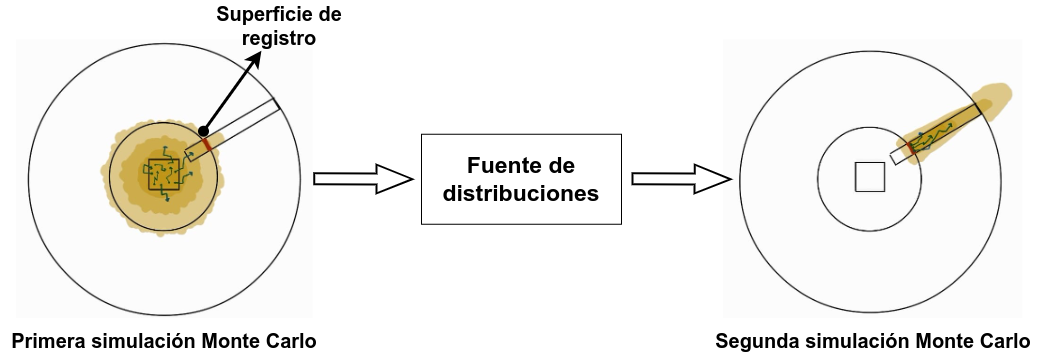
\includegraphics[width=1\linewidth]{imagens/nucleo4.png}
        % \caption{1º seminário do LIPES em 27/01/2025}
        % \label{fig:esquema1}
    \end{figure}
\end{frame}


% \begin{frame}{Motivación}
%     \begin{itemize}[itemsep=1.5em]
%         \item \textbf{Problema:} En cálculos Monte Carlo de blindaje y extracción de haces de neutrones, se necesita determinar el flujo de radiación a grandes distancias de la fuente, en zonas de bajo flujo.
%         % \item \textbf{Desafío:} El cálculo de blindajes implica evaluar flujos en regiones con niveles muy bajos, lo que complica la simulación.
%         \item \textbf{Solución:} Reducir tiempos de cómputo mediante técnicas de reducción de varianza.
%         \item \textbf{Enfoque:} Incorporar técnicas de muestreo con histogramas multidimensionales en el código de simulación Monte Carlo KDSource.
%     \end{itemize}
% \end{frame}


% \section{Introducción}
% \begin{frame}{Introducción}
%     En este trabajo se planea incorporar una:
%     \begin{itemize}[itemsep=1.5em]
%         \item Técnica de muestreo...
%         \item ... mediante histogramas multidimensionales...
%         \item ... al código de simulación de fuentes Monte Carlo KDSource.
%     \end{itemize}
% \end{frame}

% \begin{frame}{Técnica de muestreo}
%     \begin{figure}
%         \centering
%         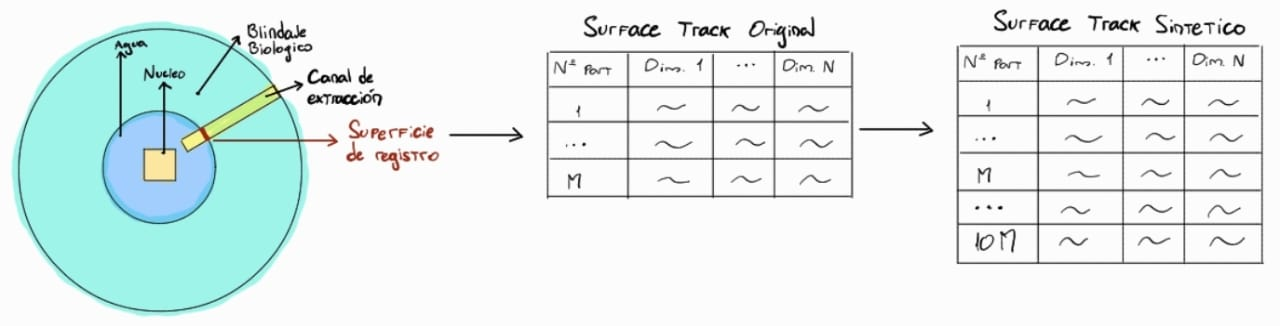
\includegraphics[width=0.95\linewidth]{imagens/esquema1.jpeg}
%         % \caption{1º seminário do LIPES em 27/01/2025}
%         \label{fig:esquema1}
%     \end{figure}

%     A partir de una simulación Monte Carlo se obtiene una lista de las partículas que atraviesan una superficie de registro.\\
%     \newline
%     Luego se genera una lista de partículas de mayor tamaño para continuar la simulación desde esa superficie en adelante.
% \end{frame}

\begin{frame}{Histogramas multidimensionales}
    \begin{figure}
        \centering
        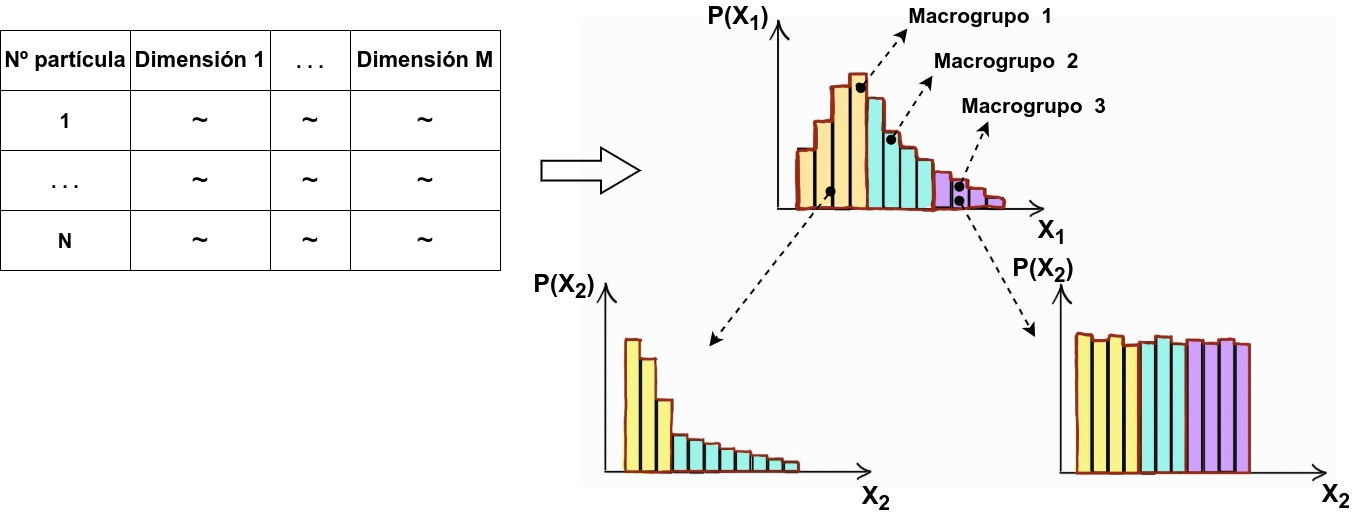
\includegraphics[width=1\linewidth]{imagens/tabla.png}
        % \caption{1º seminário do LIPES em 27/01/2025}
        \label{fig:esquema2}
    \end{figure}

    % Obtener aproximaciones de la distribución de probabilidad y correlación de las variables.
    % \textcolor{red}{Se realiza un histograma de la primera variable y se la subdivide en macro grupos. \\}
    % \textcolor{red}{Luego se realizan subsiguientes histogramas de la siguiente variable para cada macro grupo. \\}
    % \textcolor{red}{Se repite el proceso hasta formar un árbol de histogramas multidimensionales.\\}
    
    \begin{textblock*}{10cm}(1.2cm, 5.5cm) % Adjust the position and size as needed
        \textbf{Histogramas macro:}
            \begin{itemize}
                    \item Similitud por variables.
                    \item Cantidad de macrogrupos.
                    \item Límites de macrogrupos manuales. 
            \end{itemize} 
    \end{textblock*}

\end{frame}

% \begin{frame}[fragile]{Histogramas multidimensionales}
%     \textbf{Histogramas macro:}
%     \begin{itemize}
%         \item Similitud por variables.
%         \item Cantidad de macrogrupos.
%         \item Límites de macrogrupos manuales. 
%     \end{itemize} 
    
%     \vspace{2\baselineskip}
%     Input típico:

%     \begin{minted}[frame=single, linenos=false]{python}
%     orden_columnas = ['letargia', 'x', 'y', 'mu', 'phi']
%     macro_grupos = [6,5,5,4]
%     \end{minted}

% \end{frame}

\begin{frame}[fragile]{Histogramas multidimensionales}
    % Explicación de un input típico:

    \begin{minted}[frame=single, linenos=false]{python}
    orden_columnas = ['letargia', 'x', 'y', 'mu', 'phi']
    macro_grupos = [6,5,5,4]
    \end{minted}

    \begin{figure}
        \centering
        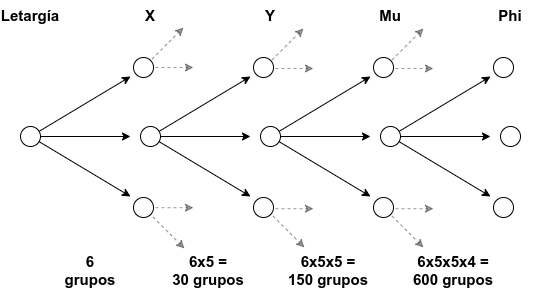
\includegraphics[width=0.6\linewidth]{imagens/grupos.png}
        % \caption{Total: 1 + 30 + 150 + 600 = 781 grupos macro en estructura de arbol.}
        \label{fig:esquema31}
    \end{figure}

    \begin{itemize}
        % \item Se obtiene un histograma macro de 6 grupos de letargia
        % \item Luego se obtienen un histograma macro de 5 grupos de x para cada grupo en letargia. \\En total 30 grupos de x.
        % \item Luego se obtienen un histograma macro de 5 grupos de y para cada grupo en x. \\En total 150 grupos de y.
        % \item Luego se obtienen un histograma macro de 4 grupos de mu para cada grupo en y. \\En total 600 grupos de mu.
        \item Total: 6 + 30 + 150 + 600 = 786 grupos macro en estructura de árbol.
    \end{itemize}
    % \newline
    % \textcolor{red}{Luego, para cada grupo macro se obtiene un histograma micro de la variable de interés.}

\end{frame}

\begin{frame}[fragile]{Histogramas multidimensionales}
    \begin{figure}
        \centering
        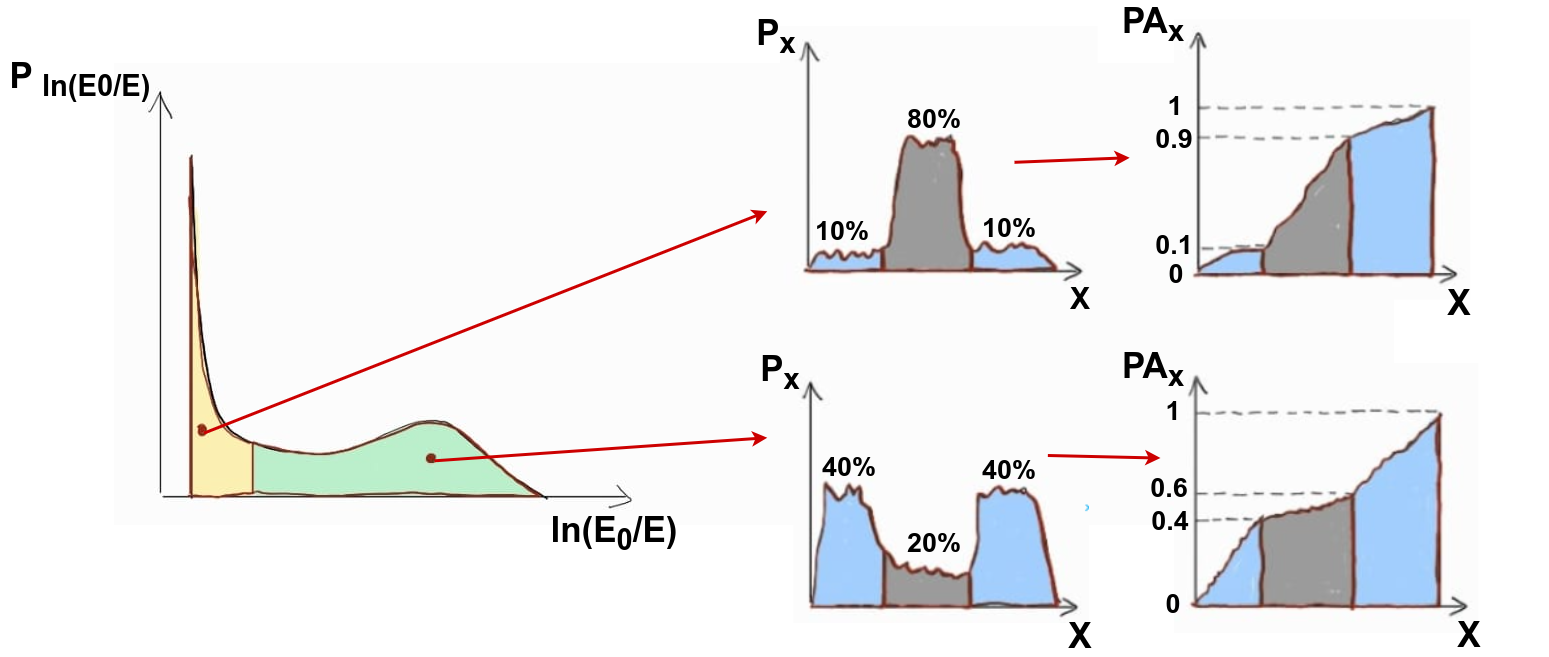
\includegraphics[width=0.93\linewidth]{imagens/esquema4.png}
        % \caption{Total: 1 + 30 + 150 + 600 = 781 grupos macro en estructura de arbol.}
        \label{fig:esquema4}
    \end{figure}
    \begin{textblock*}{10cm}(1.2cm, 6.6cm) % Adjust the position and size as needed
        \textbf{Histogramas micro:}
            \begin{itemize}
                % \item Para cada macro grupo se obtiene un histograma micro de la variable de interés.
                % \item A partir del histograma se normaliza y se obtiene la distribución de frecuencia acumulada.
                % \item La elección del número de microgrupos es un compromiso entre obtener una buena aproximación de la distribución de probabilidad y evitar reproducir el ruido estadístico.
                % \item A partir de este enfoque de macro y micro histogramas se logra aproximar la correlación intrínseca entre las variables de interés.
                \item Cantidad de microgrupos.
                \item Distribución de probabilidad de las variables.
                \item Correlación en el espacio de fases.
            \end{itemize} 
    \end{textblock*}



    % \textcolor{red}{Luego es posible muestrear listas de partículas sintéticas a partir de los histogramas multidimensionales, utilizando números pseudoaleatorios y las funciones de frecuencia acumulada.}

    % BORRADOR: tal vez poner dos esquemas de muchos y pocos micro bines. Sino ver que hacer para que no quede tan vacía
     

\end{frame}

\begin{frame}{Muestreo de partículas}
    \begin{figure}
        \centering
        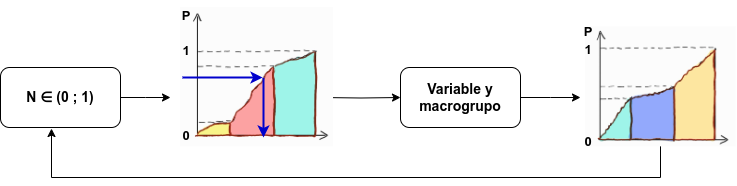
\includegraphics[width=1\linewidth]{imagens/esquema5.png}
        % \caption{Total: 1 + 30 + 150 + 600 = 781 grupos macro en estructura de arbol.}
        \label{fig:esquema5}
    \end{figure}

    \begin{itemize}
        % \item Para cada variable se genera un número pseudoaleatorio entre 0 y 1 y se interpola la inversa de la función de frecuencia acumulada para obtener el valor de la variable. 
        % \item Una vez obtenido el valor de la variable, se selecciona el macro grupo correspondiente y se obtiene la función de frecuencia acumulada correspondiente para la siguiente variable.
        % \item Se repite el proceso hasta obtener todas las variables de interés.
        % \item Se generan N partículas sintéticas y se exportan con formato .h5 para poder ser leídas como fuente por OpenMC.
        \item Comparación simulando la lista de partículas original y la lista de partículas sintéticas.
    \end{itemize}

\end{frame}

\begin{frame}{Entorno: OpenMC y KDSource}
    \begin{figure}
        \centering
        \begin{minipage}{0.35\textwidth}
            \centering
            
\includegraphics[width=\linewidth]{imagens/openmc.png}
            % \caption{Esquema 3}
            \label{fig:openmc}
        \end{minipage}\hfill
        \begin{minipage}{0.35\textwidth}
            \centering
            
\includegraphics[width=\linewidth]{imagens/esquema3.png}
            % \caption{Otra imagen}
            \label{fig:esquema3}
        \end{minipage}
    \end{figure}

    \begin{columns}[t]
        \column{0.45\textwidth}
            \begin{itemize}
                \item Código Monte Carlo open source.
                \item Transporte de neutrones y fotones.
            \end{itemize}
        \column{0.45\textwidth}
            \begin{itemize}
                \item Inicialmente para simular fuentes de neutrones y fotones mediante \textit{kernel density estimation}.
                \item En desarrollo para incorporar histogramas multidimensionales.
                \item Originado en trabajos de grado y posgrado en el Instituto Balseiro.
            \end{itemize}
    \end{columns}
\end{frame}

% \section{Estado actual}
% \begin{frame}{Estado actual}
%     \begin{itemize}
%         \item Interiorización del problema y de las técnicas a incorporar.
%         \item Método para la aproximación de la distribución de probabilidad de las variables de interés a través de histogramas multidimensionales en Python. 
%         \item Método para la generación de listas de partículas sintéticas a partir de los histogramas multidimensionales en Python. 
%         \item Resultados preliminares en un canal de extracción de neutrones.
%         % \item \textcolor{red}{Todo el trabajo se ha realizado para neutrones, excluyendo los fotones.}
%     \end{itemize}
%     % \begin{figure}
%     %     \centering
%     %     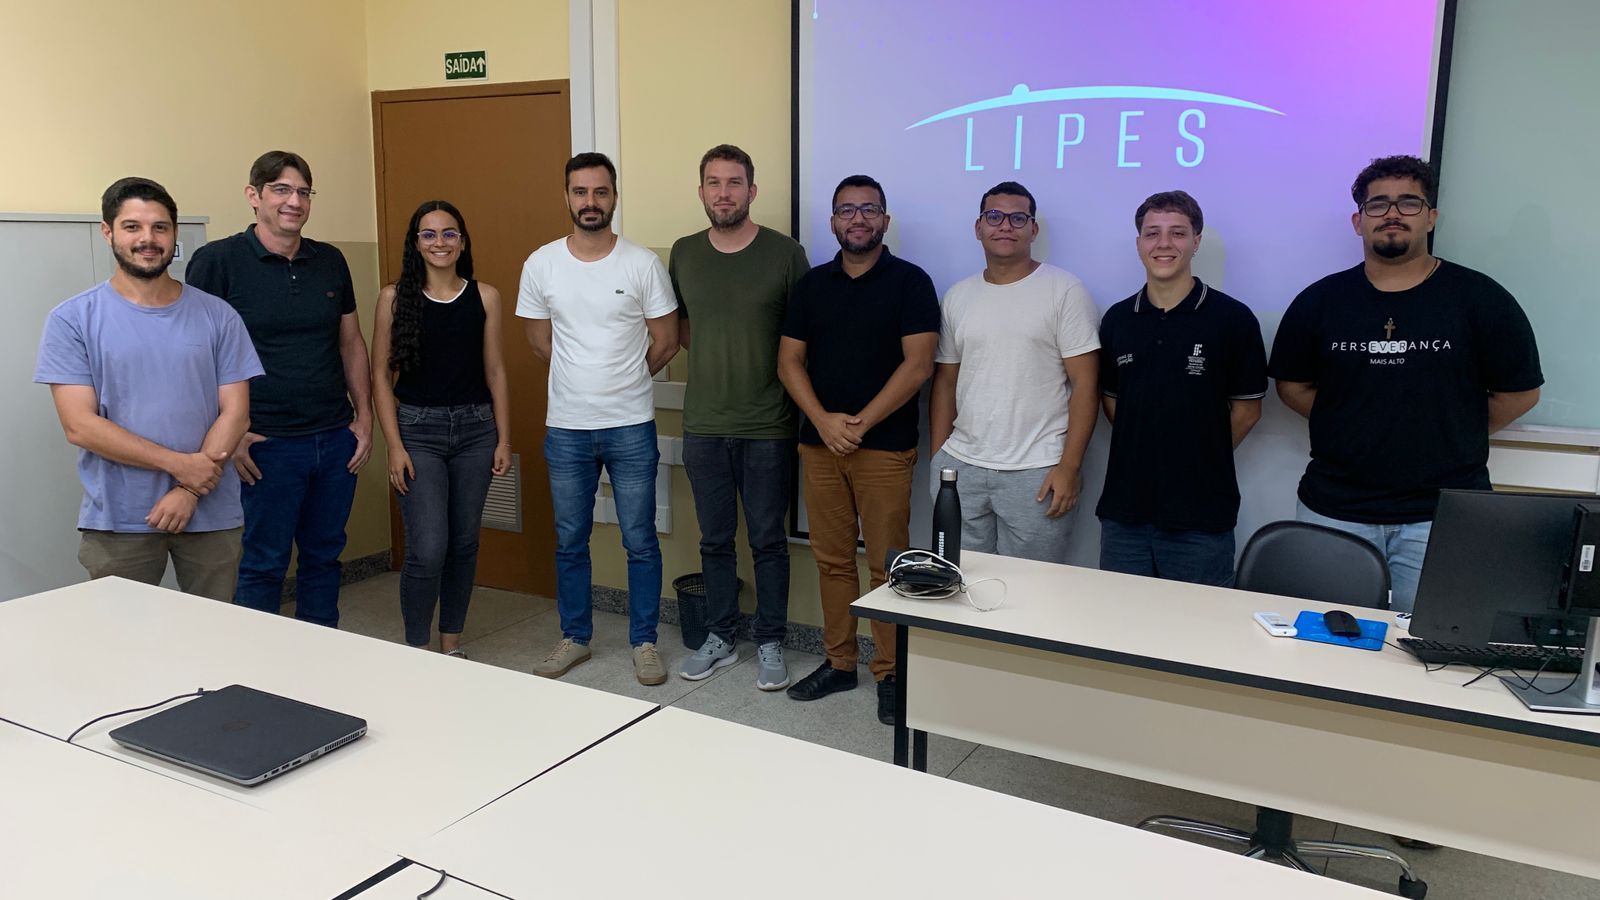
\includegraphics[width=0.6\linewidth]{imagens/1_seminario_LIPES.jpeg}
%     %     % \caption{1º seminário do LIPES em 27/01/2025}
%     %     \label{fig:1semlipes}
%     % \end{figure}

% \end{frame}



\section{Resultados preliminares}
\begin{frame}{Ejemplo de aplicación}
    % \begin{figure}
    %     \centering
    %     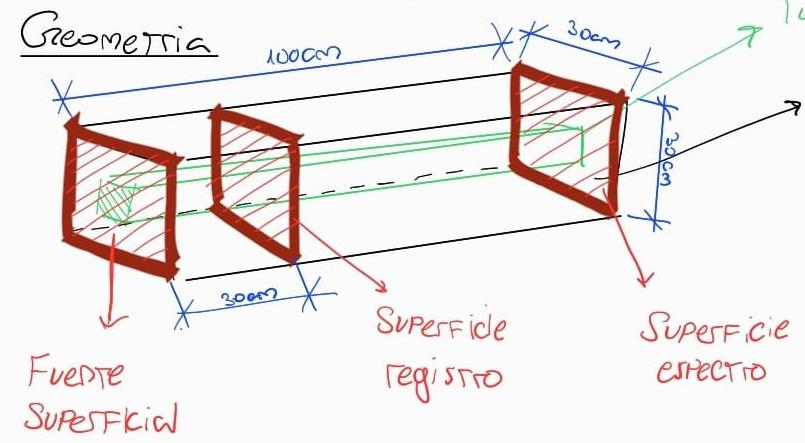
\includegraphics[width=0.55\linewidth]{imagens/croquis1.jpeg}
    %     % \caption{Total: 1 + 30 + 150 + 600 = 781 grupos macro en estructura de arbol.}
    %     \label{fig:croquis1}
    % \end{figure}
    
    % \centering
    % Características de la fuente:
    % \begin{itemize}
    %     \centering
    %     \item Monoenergética de $1 MeV$
    %     \item Uniforme en el plano $XY$
    %     \item Colimada en $\mu = 1$ 
    % \end{itemize}

    \begin{columns}
        \column{0.7\textwidth}
        \begin{figure}
            \centering
            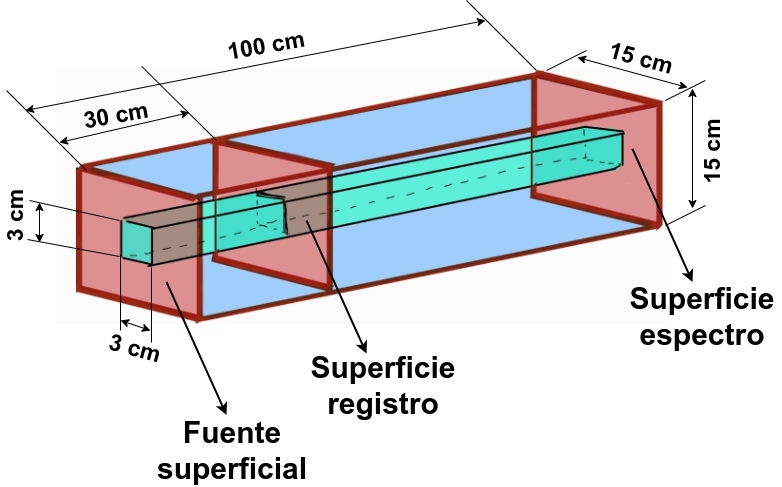
\includegraphics[width=\linewidth]{imagens/croquis1.png}
            \label{fig:croquis1}
        \end{figure}
        
        \column{0.35\textwidth}
        Características de la fuente:
        \begin{itemize}
            \item Monoenergética de $1 \, MeV$
            \item Uniforme en el plano $XY$
            \item Colimada en $\mu = 1$ 
        \end{itemize}
    \end{columns}

\end{frame}

\begin{frame}{Ejemplo de aplicación: Flujo}
    \begin{figure}
        \centering
        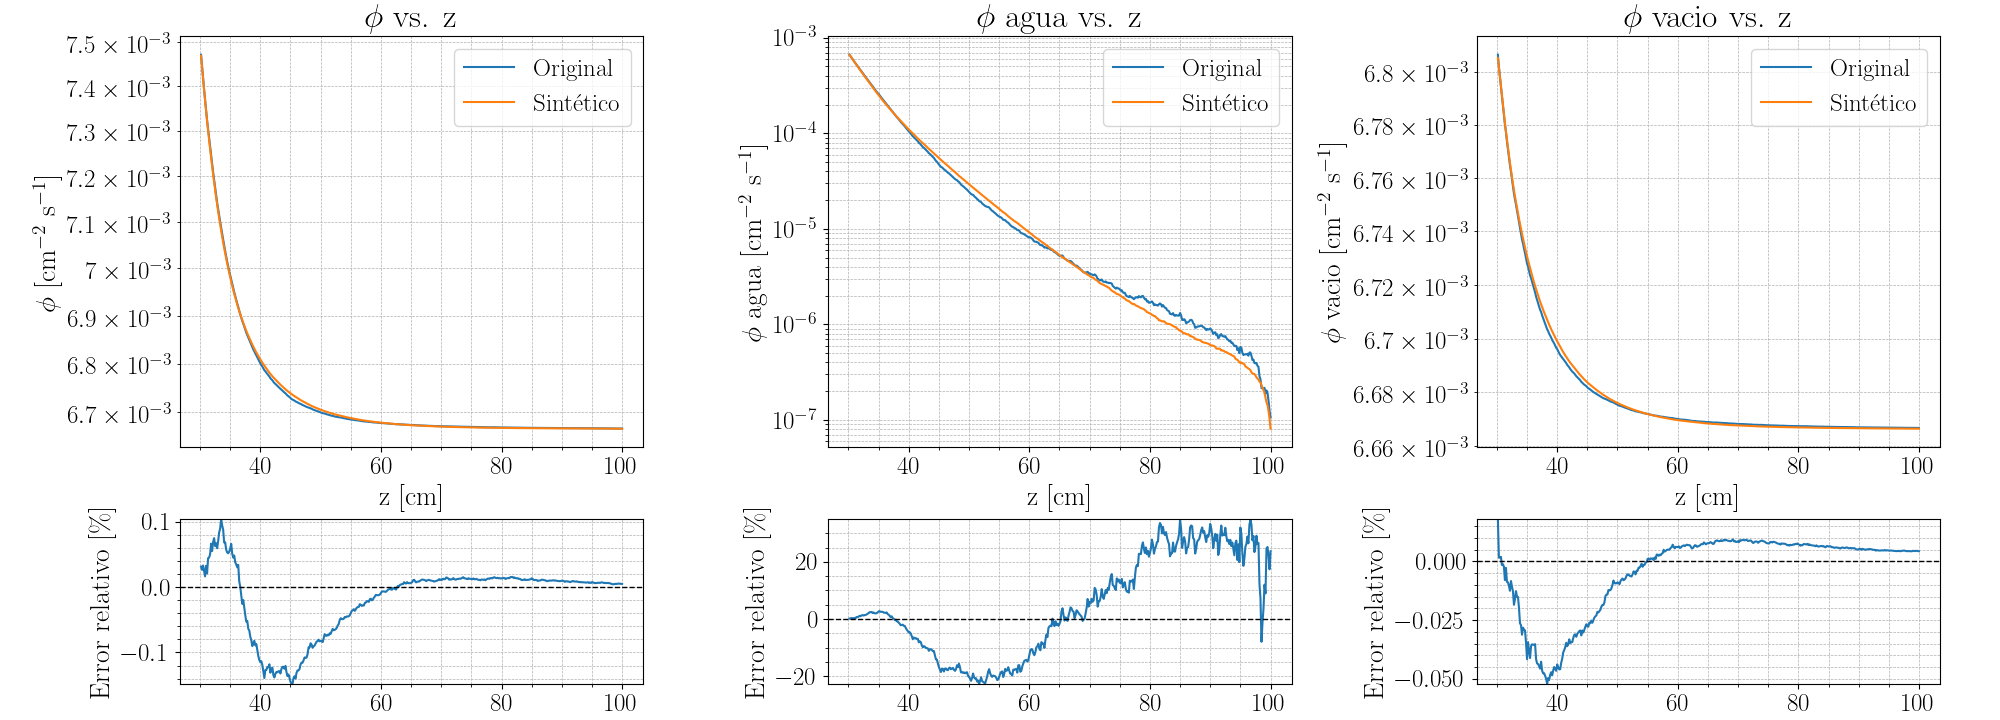
\includegraphics[width=1\linewidth]{imagens/resultados_flujo.png}
        \label{fig:flujos.png}
    \end{figure}
    % \textcolor{red}{Falta poner los datos de esta simulación. Pero no los puse porque después voy a hacer estos gráficos de vuelta y tal vez use otros inputs.}
    

\end{frame}

\begin{frame}{Ejemplo de aplicación: Espectro}
    
    \begin{figure}
        \centering
        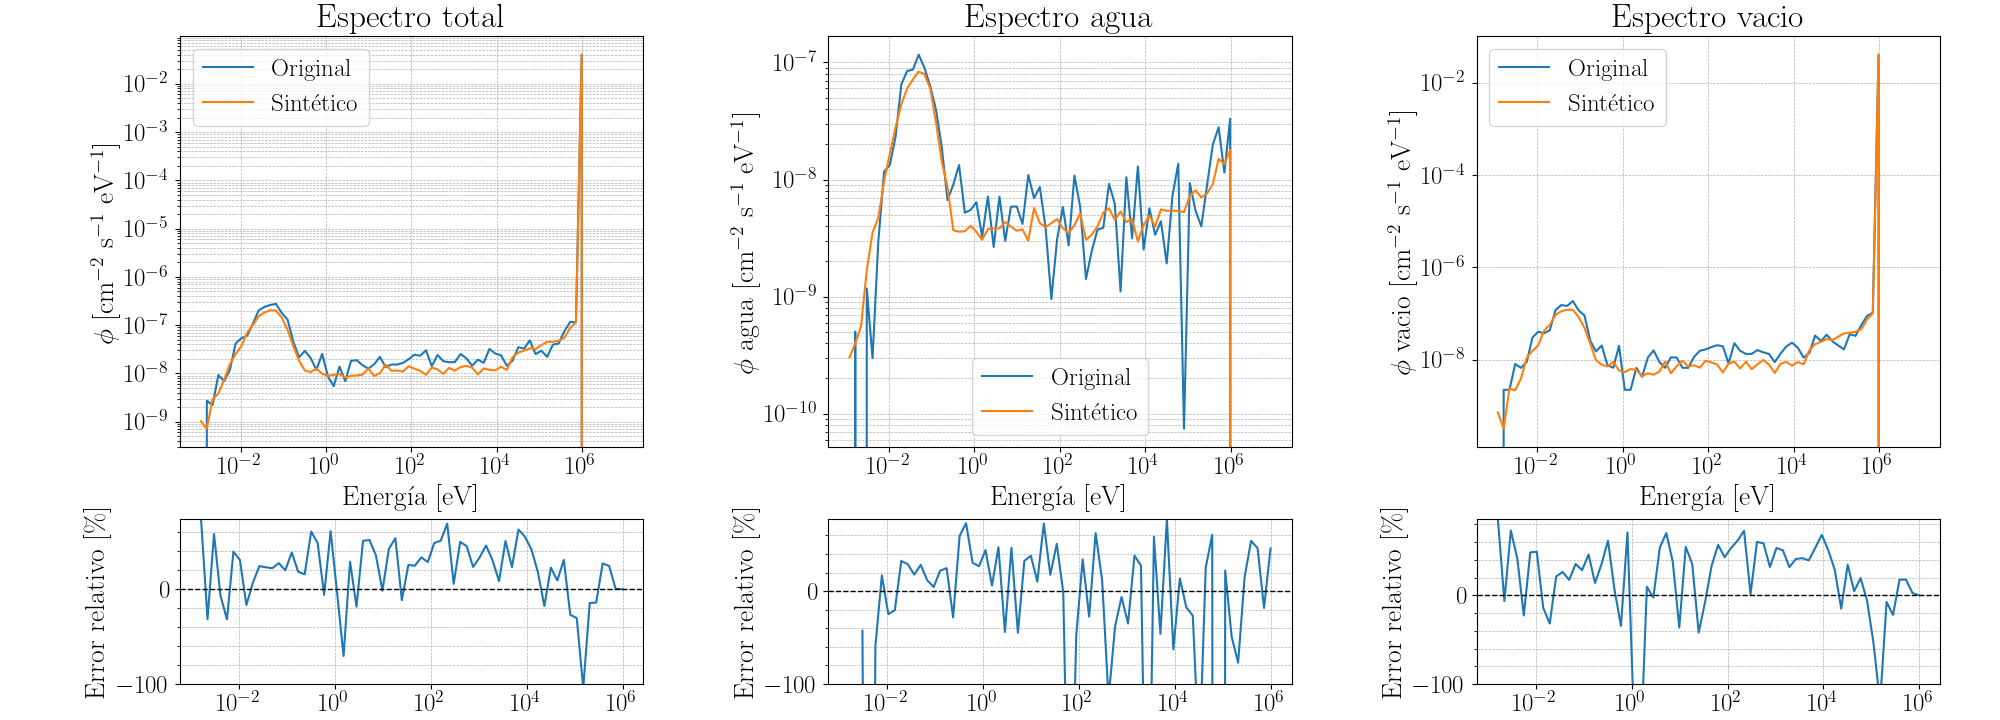
\includegraphics[width=1\linewidth]{imagens/resultados_espectro.png}
        \label{fig:espectros.png}
    \end{figure}

\end{frame}

% \begin{frame}{Resultados preliminares: Ejemplo de aplicacion}
%     Entre ellos comentar diferencias entre incorporar o no los limites manuales de los macrogrupos (geometricos y en letargia). \\
%     Ademas comentar diferencias entre diferente cantidad de micro y macrogrupos. Y tambien entre mayor o menor cantidad de particulas registradas.\\
%     Ademas comentar del tubo de vacio y caracteristicas delticas de la fuente que estamos utilizando (delta en mu y en letargia).\\
%     Ademas comentar que miramos el flujo a traves de la dimension de propagacion (total, agua y vacio) y que se observa el espectro al final del tubo (total, agua y vacio).

    

% \end{frame}

\section{Conclusiones}
\begin{frame}{Conclusiones preliminares}
    \begin{itemize}
        \item Se realizó una interiorización del problema y de las técnicas para abordarlo.\\
        \item Se implementó un método de muestreo mediante histogramas multidimensionales en Python.\\
        \item Se obtuvieron resultados preliminares de la aplicación del método propuesto.\\
            \begin{itemize}
            \item Se encontró que existe un compromiso en la elección de la cantidad de macro y micro bines para obtener mejores resultados.\\
            \item Se incorporaron límites manuales en las interfaces vacío/agua, así como para separar partículas con colisiones de aquellas sin colisiones.\\
            \end{itemize}
        % \item \textcolor{red}{Comentar que es relevante porque luego de un colimador el haz es bastante monodireccional.}\\
        % \item Ventaja relativa frente al método basado en KDE. \\
    
    \end{itemize}

\end{frame}

% \section{Trabajo futuro}
\begin{frame}{Trabajo futuro}

    \begin{itemize}
        \item Incorporar método de muestreo basado en histogramas multidimensionales al entorno KDSource.\\
        \item Incorporar algoritmo de selección de parámetros automáticos.\\
        % \item Incorporar a la API de KDSource el método de muestreo de partículas sintéticas. \\
        \item Aplicar el método a una simulación del CHOPPER en el conducto N5 del RA6. \\
    \end{itemize}


\end{frame}

% \section{Fin}
% \section*{Fin}
\begin{frame}{FIN}
    \centering
    \Huge{FIN\\}
    \vspace{1cm}
    \LARGE{¿Preguntas?}
\end{frame}

% \section{Código}
% \begin{frame}[fragile]{Código}
% \begin{minted}{python}
% from qiskit import QuantumRegister, QuantumCircuit
% from numpy import pi

% qreg_q = QuantumRegister(2, 'q')
% circuit = QuantumCircuit(qreg_q)

% circuit.h(qreg_q[0])
% circuit.cx(qreg_q[0], qreg_q[1])
% \end{minted}
% \end{frame}

% \section{Citação}
% \begin{frame}{Citação}
%     \begin{itemize}
%         \item De acordo com \citeonline{fernandes2017} ...
%         \item ... lorem ipsum \cite{fernandes2023}.
%     \end{itemize}
% \end{frame}

% FIM DO CONTEÚDO -----------------------------------------------------------------

% NÃO REMOVA! 
% Comentarios:  benchmark GODIVA para anexo. 
                % Tildes
                % resultados preliminares
                % unidades
\section{Referências}
\begin{frame}[allowframebreaks]
    \addtocounter{framenumber}{-1}
    \frametitle{Referências}
    \scriptsize
    % \bibliographystyle{abntex2-alf-en}  % mude para qualquer arquivo .bst
    \bibliography{referencias}
\end{frame}     
\end{document}